% !TEX encoding = UTF-8 Unicode
% !TEX TS-program = xelatex 
\begin{QUESTIONS}
    \begin{QUESTION}
        \begin{ExamInfo}{099}{學測}{單選}{1}
        \end{ExamInfo}
        \begin{ExamAnsRateInfo}{49}{82}{49}{16}
        \end{ExamAnsRateInfo}
        \begin{QBODY}
			若數列 $a_1,a_2,\dots,a_k,\dots,a_{10}$ 中每一項皆為 1 或 $-1$,則 $a_1 +a_2 +\cdots +a_k +\cdots+a_{10}$ 之值有多少種可能?
			\begin{QOPS} 
				\QOP 10    
				\QOP 11 
				\QOP $P^{10}_2$    
				\QOP $C^{10}_2$    
				\QOP $2^{10}$
			\end{QOPS}
        \end{QBODY}
        \begin{QFROMS}
        \end{QFROMS}
        \begin{QTAGS}\QTAG{B2C2排列組合}\end{QTAGS}
        \begin{QANS}
            (2)
        \end{QANS}
        \begin{QSOLLIST}
        \end{QSOLLIST}
        \begin{QEMPTYSPACE}
        \end{QEMPTYSPACE}
    \end{QUESTION}
    \begin{QUESTION}
        \begin{ExamInfo}{099}{學測}{單選}{2}
        \end{ExamInfo}
        \begin{ExamAnsRateInfo}{58}{83}{62}{29}
        \end{ExamAnsRateInfo}
        \begin{QBODY}
			已知 $a,b$ 為整數且行列式 $\left| \begin{array}{cc} 5 & a \\ b & 7  \end{array}\right| =4$,
			則絕對值 $|a+b|$ 為何? 
			\begin{QOPS} 
				\QOP 16 
				\QOP 31 
				\QOP 32 
				\QOP 39 
				\QOP 條件不足,無法確定。
			\end{QOPS}
        \end{QBODY}
        \begin{QFROMS}
        \end{QFROMS}
        \begin{QTAGS}\QTAG{B3C3平面向量}\end{QTAGS}
        \begin{QANS}
            (3)
        \end{QANS}
        \begin{QSOLLIST}
        \end{QSOLLIST}
        \begin{QEMPTYSPACE}
        \end{QEMPTYSPACE}
    \end{QUESTION}
    \begin{QUESTION}
        \begin{ExamInfo}{099}{學測}{單選}{3}
        \end{ExamInfo}
        \begin{ExamAnsRateInfo}{55}{84}{62}{19}
        \end{ExamAnsRateInfo}
        \begin{QBODY}
			箱中有三顆紅球與三顆白球。一摸彩遊戲是從箱中隨機同時抽出兩顆球。如果抽出的兩球顏色不同,則得獎金100 元;如果兩球顏色相同,則無獎金。請問此遊戲獎金的期望值為何?
			\begin{QOPS} 
				\QOP 20 元 
				\QOP 30 元 
				\QOP 40 元 
				\QOP 50 元 
				\QOP 60 元
			\end{QOPS}
        \end{QBODY}
        \begin{QFROMS}
        \end{QFROMS}
        \begin{QTAGS}\QTAG{B5C1機率與統計}\end{QTAGS}
        \begin{QANS}
            (5)
        \end{QANS}
        \begin{QSOLLIST}
        \end{QSOLLIST}
        \begin{QEMPTYSPACE}
        \end{QEMPTYSPACE}
    \end{QUESTION}
    \begin{QUESTION}
        \begin{ExamInfo}{099}{學測}{單選}{4}
        \end{ExamInfo}
        \begin{ExamAnsRateInfo}{33}{61}{25}{13}
        \end{ExamAnsRateInfo}
        \begin{QBODY}
			坐標平面上給定兩點 $A(1,0)$ 與 $B(0,1)$,又考慮另外三點 $P(\pi,1)$、$Q(-3,6)$ 與 $R(2,\log_4 32)$。令 $\triangle PAB$ 的面積為 $p$ 、 $\triangle QAB$ 的面積為 $q$ 、 $\triangle RAB$ 的面積為 r 。請問下列哪一個選項是正確的? 
			\begin{QOPS} 
				\QOP $p< q< r$ 
				\QOP $p < r <q$ 
				\QOP $q<p < r$ 
				\QOP $q<r<p$ 
				\QOP $r<q<p$。
			\end{QOPS}
        \end{QBODY}
        \begin{QFROMS}
        \end{QFROMS}
        \begin{QTAGS}\QTAG{B3C1三角}\end{QTAGS}
        \begin{QANS}
            (1)
        \end{QANS}
        \begin{QSOLLIST}
        \end{QSOLLIST}
        \begin{QEMPTYSPACE}
        \end{QEMPTYSPACE}
    \end{QUESTION}
    \begin{QUESTION}
        \begin{ExamInfo}{099}{學測}{單選}{5}
        \end{ExamInfo}
        \begin{ExamAnsRateInfo}{26}{46}{20}{12}
        \end{ExamAnsRateInfo}
        \begin{QBODY}
			在密閉的實驗室中, 開始時有某種細菌 1 千隻,並且以每小時增加 $8\%$ 的速率繁殖。 如果依此速率持續繁殖,則 100 小時後細菌的數量最接近下列哪一個選項?
			\begin{QOPS} 
				\QOP 9 千隻 
				\QOP 108 千隻 
				\QOP 2200 千隻
				\QOP 3200 千隻 
				\QOP 32000 千隻
			\end{QOPS}
        \end{QBODY}
        \begin{QFROMS}
        \end{QFROMS}
        \begin{QTAGS}\QTAG{B1C3指對數函數}\end{QTAGS}
        \begin{QANS}
            (3)
        \end{QANS}
        \begin{QSOLLIST}
        \end{QSOLLIST}
        \begin{QEMPTYSPACE}
        \end{QEMPTYSPACE}
    \end{QUESTION}
    \begin{QUESTION}
        \begin{ExamInfo}{099}{學測}{單選}{6}
        \end{ExamInfo}
        \begin{ExamAnsRateInfo}{49}{70}{53}{24}
        \end{ExamAnsRateInfo}
        \begin{QBODY}
			坐標空間中 $O$ 為原點,點 $A$ 的坐標為  $(1,2,1)$ 。設 $S$ 是以  $O$ 為球心、 $4$ 為半徑的球面。請問在 $S$ 上滿足內積 $\lvec{OA} \cdot \lvec{ OP} = 6$ 的所有點 $P$ 所成的圖形為何?
			\begin{QOPS} 
				\QOP 空集合 
				\QOP 一個點 
				\QOP 兩個點 
				\QOP 一個圓 
				\QOP 兩個圓 
			\end{QOPS}
        \end{QBODY}
        \begin{QFROMS}
        \end{QFROMS}
        \begin{QTAGS}\QTAG{B4C1空間向量}\end{QTAGS}
        \begin{QANS}
            (4)
        \end{QANS}
        \begin{QSOLLIST}
        \end{QSOLLIST}
        \begin{QEMPTYSPACE}
        \end{QEMPTYSPACE}
    \end{QUESTION}
    \begin{QUESTION}
        \begin{ExamInfo}{099}{學測}{單選}{7}
        \end{ExamInfo}
        \begin{ExamAnsRateInfo}{33}{65}{22}{12}
        \end{ExamAnsRateInfo}
        \begin{QBODY}
			令橢圓 $\Gamma_1 : \frac{x^2}{5^2} + \frac{y^2}{3^2} =1$、$\Gamma_2 : \frac{x^2}{5^2} + \frac{y^2}{3^2} =2$, $\Gamma_3 : \frac{x^2}{5^2} + \frac{y^2}{3^2} =\frac{2x}{5}$ 的長軸方別為 $l_1$, $l_2$, $l_3$。請問下列哪一個選項是正確的?
			\begin{QOPS} 
				\QOP $l_1=l_2=l_3$ 
				\QOP $l_1=l_2<l_3$
				\QOP $l_1<l_2<l_3$ 
				\QOP $l_1=l_3<l_2$ 
				\QOP $l_1<l_2<l_3$ 。
			\end{QOPS}
        \end{QBODY}
        \begin{QFROMS}
        \end{QFROMS}
        \begin{QTAGS}\QTAG{B4C4二次曲線}\end{QTAGS}
        \begin{QANS}
            (4)
        \end{QANS}
        \begin{QSOLLIST}
        \end{QSOLLIST}
        \begin{QEMPTYSPACE}
        \end{QEMPTYSPACE}
    \end{QUESTION}
\end{QUESTIONS}
\begin{QUESTIONS}
    \begin{QUESTION}
        \begin{ExamInfo}{099}{學測}{多選}{8}
        \end{ExamInfo}
        \begin{ExamAnsRateInfo}{39}{72}{29}{16}
        \end{ExamAnsRateInfo}
        \begin{QBODY}
			設 $\theta_1,\theta_2,\theta_3,\theta_4$ 分別為第一、第二、第三、第四象限角,且都介於 $0$ 和  $2\pi$ 之間。已知 $|\cos \theta_{1}| =|\cos \theta_{2}| =|\cos \theta_{3}| =|\cos \theta_{4}| =\frac{1}{3}$,請問下列哪些選項是正確的?
			\begin{QOPS} 
				\QOP $\theta_{1} < \frac{\pi}{4}$ 
				\QOP $\theta_{1} + \theta_{2} = \pi$
				\QOP $ \cos \theta_{3}  =-\frac{1}{3}$ 
				\QOP $\sin\theta_{4} = \frac{2\sqrt{2}}{3}$
				\QOP $\theta_{4} = \theta_{3} + \frac{\pi}{2}$ 
			\end{QOPS}
        \end{QBODY}
        \begin{QFROMS}
        \end{QFROMS}
        \begin{QTAGS}\QTAG{B3C1三角}\end{QTAGS}
        \begin{QANS}
            (2)(3)
        \end{QANS}
        \begin{QSOLLIST}
        \end{QSOLLIST}
        \begin{QEMPTYSPACE}
        \end{QEMPTYSPACE}
    \end{QUESTION}
    \begin{QUESTION}
        \begin{ExamInfo}{099}{學測}{多選}{9}
        \end{ExamInfo}
        \begin{ExamAnsRateInfo}{24}{50}{14}{8}
        \end{ExamAnsRateInfo}
        \begin{QBODY}
			下列哪些方程式有實數解?
			\begin{QOPS} 
				\QOP $x^3 +x -1=0$ 
				\QOP $2^x +2^{-x} =0$ 
				\QOP $\log_2 x+ \log_x 2=1$ 
				\QOP $\sin{x}+ \cos{2x}=3$
				\QOP $4\sin{x}+3\cos{x}=\frac{9}{2}$.
			\end{QOPS}
        \end{QBODY}
        \begin{QFROMS}
        \end{QFROMS}
        \begin{QTAGS}\QTAG{綜合}\end{QTAGS}
        \begin{QANS}
            (1)(5)
        \end{QANS}
        \begin{QSOLLIST}
        \end{QSOLLIST}
        \begin{QEMPTYSPACE}
        \end{QEMPTYSPACE}
    \end{QUESTION}
    \begin{QUESTION}
        \begin{ExamInfo}{099}{學測}{多選}{10}
        \end{ExamInfo}
        \begin{ExamAnsRateInfo}{34}{53}{33}{16}
        \end{ExamAnsRateInfo}
        \begin{QBODY}
			設 $a_{1},a_{2},\cdots,a_{n}$ 為一實數數列,
			且對所有的正整數 $n$ 滿足 $a_{n+1} = n(n+1) - a_{n}$。
			請問下列哪些選項是正確的?
			\begin{QOPS} 
				\QOP 如果 $a_{1}=1$,則 $a_{2}=1$
				\QOP 如果 $a_{1}$ 是整數,則此數列的每一項都是整數
				\QOP 如果 $a_{1}$ 是無理數,則此數列的每一項都是無理數
				\QOP $a_{1} \leq a_{2} \leq  \cdots \leq a_{2n} \leq \cdots $ ($n$ 為正整數)
				\QOP 如果 $a_{1}$ 是奇數,則 
			$a_{k+2}, a_{k+4} ,  \cdots \leq a_{k+2n} \leq \cdots $ 都是奇數($n$ 為正整數)
			\end{QOPS}
        \end{QBODY}
        \begin{QFROMS}
        \end{QFROMS}
        \begin{QTAGS}\QTAG{B2C1數列級數}\end{QTAGS}
        \begin{QANS}
            (2)(3)(4)
        \end{QANS}
        \begin{QSOLLIST}
        \end{QSOLLIST}
        \begin{QEMPTYSPACE}
        \end{QEMPTYSPACE}
    \end{QUESTION}
    \begin{QUESTION}
        \begin{ExamInfo}{099}{學測}{多選}{11}
        \end{ExamInfo}
        \begin{ExamAnsRateInfo}{17}{25}{16}{10}
        \end{ExamAnsRateInfo}
        \begin{QBODY}
			坐標空間中,直線 $L$ 上距離點 $Q$ 最近的點稱為 $Q$ 在 $L$ 上的投影點。 已知 $L$ 為平面 $2x-y=2$ 上通過點 $(2, 2, 2)$ 的一直線。請問下列哪些選項中的點可能是原點 $O$ 在 $L$ 上的投影點? 
			\begin{QOPS} 
				\QOP (2,2,2) 
				\QOP (2,0,2) 
				\QOP $(\frac{4}{5},-\frac{2}{5},0)$ 
				\QOP $(\frac{4}{5},-\frac{2}{5},-2)$ 
				\QOP $(\frac{8}{9},-\frac{2}{9},-\frac{2}{9})$
			\end{QOPS}
        \end{QBODY}
        \begin{QFROMS}
        \end{QFROMS}
        \begin{QTAGS}\QTAG{B4C1空間向量}\end{QTAGS}
        \begin{QANS}
            (1)(3)(5)
        \end{QANS}
        \begin{QSOLLIST}
        \end{QSOLLIST}
        \begin{QEMPTYSPACE}
        \end{QEMPTYSPACE}
    \end{QUESTION}
    \begin{QUESTION}
        \begin{ExamInfo}{099}{學測}{多選}{12}
        \end{ExamInfo}
        \begin{ExamAnsRateInfo}{21}{37}{16}{10}
        \end{ExamAnsRateInfo}
        \begin{QBODY}
			想要了解台灣的公民對某議題支持的程度所作的抽樣調查,依性別區分,所得結果如下表:
			\begin{center}
				\begin{tabular}{|c|c|c|}
					\hline
					& 女性公民& 男性公民 \\
					\hline
					贊成此議題的比例 $\hat{p}$ & 0.52 &  0.59 \\\hline
					$\hat{p}$ 的標準差   $\sqrt{\frac{\hat{p}(1-\hat{p})}{n}}$ &  0.02 & 0.04 \\\hline
				\end{tabular}
			\end{center}
			
			請問從此次抽樣結果可以得到下列哪些推論?

			\begin{QOPS} 
				\QOP 全台灣男性公民贊成此議題的比例大於女性公民贊成此議題的比例
				\QOP 在 $95\%$ 的信心水準之下,全台灣女性公民贊成此議題之比例的信賴區間為
			$[0.48,0.56]$ (計算到小數點後第二位,以下四捨五入)
				\QOP 此次抽樣的女性公民數少於男性公民數
				\QOP 如果不區分性別,此次抽樣贊成此議題的比例 $\hat{p}$ 介於 0.52 與 0.59 之間
				\QOP 如果不區分性別,此次抽樣 $\hat{p}$ 的標準差 $\sqrt{\frac{\hat{p}(1-\hat{p})}{n}}$ 介於 0.02 與 0.04 之間
			\end{QOPS}
        \end{QBODY}
        \begin{QFROMS}
        \end{QFROMS}
        \begin{QTAGS}\QTAG{B5C1機率與統計}\end{QTAGS}
        \begin{QANS}
            (2)(4)
        \end{QANS}
        \begin{QSOLLIST}
        \end{QSOLLIST}
        \begin{QEMPTYSPACE}
        \end{QEMPTYSPACE}
    \end{QUESTION}
\end{QUESTIONS}
\begin{QUESTIONS}
    \begin{QUESTION}
        \begin{ExamInfo}{099}{學測}{填充}{A}
        \end{ExamInfo}
        \begin{ExamAnsRateInfo}{29}{64}{19}{4}
        \end{ExamAnsRateInfo}
        \begin{QBODY}
			坐標平面上有一個平行四邊形 $ABCD$, 其中點 $A$ 的坐標為 (2,1), 點 $B$ 的坐標為 $(8, 2)$,點 $C$ 在第一象限且知其 $x$ 坐標為 $12$。若平行四邊形 $ABCD$ 的面積等於 38 平方單位,則點 $D$ 的坐標為 $\TCNBOX{(\TCN,\TCN)}$。
        \end{QBODY}
        \begin{QFROMS}
        \end{QFROMS}
        \begin{QTAGS}\QTAG{B3C3平面向量}\end{QTAGS}
        \begin{QANS}
            $(6,8)$
        \end{QANS}
        \begin{QSOLLIST}
        \end{QSOLLIST}
        \begin{QEMPTYSPACE}
        \end{QEMPTYSPACE}
    \end{QUESTION}
    \begin{QUESTION}
        \begin{ExamInfo}{099}{學測}{填充}{B}
        \end{ExamInfo}
        \begin{ExamAnsRateInfo}{29}{71}{15}{1}
        \end{ExamAnsRateInfo}
        \begin{QBODY}
			設 $f(x)$ 為滿足下列條件的最低次實係數多項式: $f(x)$ 最高次項的係數為 1,且 $3 - 2i$, $i$, 5 皆為方程式 $f(x)=0$ 的解(其中$i^2 =-1$),則 $f(x)$ 之常數項為	$\TCNBOX{\TCN\TCN\TCN}$。
        \end{QBODY}
        \begin{QFROMS}
        \end{QFROMS}
        \begin{QTAGS}\QTAG{B1C2多項式函數}\end{QTAGS}
        \begin{QANS}
            $-65$
        \end{QANS}
        \begin{QSOLLIST}
        \end{QSOLLIST}
        \begin{QEMPTYSPACE}
        \end{QEMPTYSPACE}
    \end{QUESTION}
    \begin{QUESTION}
        \begin{ExamInfo}{099}{學測}{填充}{C}
        \end{ExamInfo}
        \begin{ExamAnsRateInfo}{26}{53}{22}{3}
        \end{ExamAnsRateInfo}
        \begin{QBODY}
			有一個兩列三行的表格如右下圖。在六個空格中分別填入 1、2、3、4、5、6(不得重複),則 1、2 這兩個數在同一行或同一列的方法有 $\TCNBOX{\TCN\TCN\TCN}$ 種。

			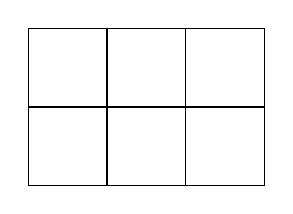
\begin{tikzpicture}
				\foreach \x in {0,1,2,3}
					\draw (\x,0) to (\x,2);
				\foreach \y in {0,1,2}
					\draw (0,\y) to (3,\y);	
			\end{tikzpicture}
        \end{QBODY}
        \begin{QFROMS}
        \end{QFROMS}
        \begin{QTAGS}\QTAG{B2C2排列組合}\end{QTAGS}
        \begin{QANS}
            $432$
        \end{QANS}
        \begin{QSOLLIST}
        \end{QSOLLIST}
        \begin{QEMPTYSPACE}
        \end{QEMPTYSPACE}
    \end{QUESTION}
    \begin{QUESTION}
        \begin{ExamInfo}{099}{學測}{填充}{D}
        \end{ExamInfo}
        \begin{ExamAnsRateInfo}{41}{71}{42}{10}
        \end{ExamAnsRateInfo}
        \begin{QBODY}
			設實數 $a>0$,若 $x$, $y$ 的方程組 $\left\{ \begin{array}{rcl} 2x-y & = &1 \\ x-2y &=&a \\ x-ay &= & 122 \end{array}\right.$有解,則$a=\TCNBOX{\TCN\TCN}$ 。
        \end{QBODY}
        \begin{QFROMS}
        \end{QFROMS}
        \begin{QTAGS}\QTAG{B4C3矩陣}\end{QTAGS}
        \begin{QANS}
            $14$
        \end{QANS}
        \begin{QSOLLIST}
        \end{QSOLLIST}
        \begin{QEMPTYSPACE}
        \end{QEMPTYSPACE}
    \end{QUESTION}
    \begin{QUESTION}
        \begin{ExamInfo}{099}{學測}{填充}{E}
        \end{ExamInfo}
        \begin{ExamAnsRateInfo}{31}{75}{17}{1}
        \end{ExamAnsRateInfo}
        \begin{QBODY}
			直角三角形 $ABD$ 中, $\angle A$ 為直角, $C$ 為 $AD$ 邊上的點。
			已知 $\overline{BC} = 6$ , $\overline{AB} = 5$ , $\angle ABD = 2 \angle ABC$ ,則 $\overline{BD} = \TCNBOX{\FR{\TCN\TCN}{\TCN}}$。
        \end{QBODY}
        \begin{QFROMS}
        \end{QFROMS}
        \begin{QTAGS}\QTAG{B3C1三角}\end{QTAGS}
        \begin{QANS}
            $\dfrac{90}{7}$
        \end{QANS}
        \begin{QSOLLIST}
        \end{QSOLLIST}
        \begin{QEMPTYSPACE}
        \end{QEMPTYSPACE}
    \end{QUESTION}
    \begin{QUESTION}
        \begin{ExamInfo}{099}{學測}{填充}{F}
        \end{ExamInfo}
        \begin{ExamAnsRateInfo}{15}{40}{4}{1}
        \end{ExamAnsRateInfo}
        \begin{QBODY}
			設 $a$、$b$ 為實數。已知坐標平面上拋物線 $y=x^2 +ax+b$ 與 $x$ 軸交於 $P$、$Q$ 兩點,且 $\overline{PQ}=7$。 若拋物線 $y=x^2 +ax+(b+2)$ 與 $x$ 軸的兩交點為 $R$、$S$,則 $\overline{RS}=\TCNBOX{\sqrt{\TCN\TCN}}$ 。
        \end{QBODY}
        \begin{QFROMS}
        \end{QFROMS}
        \begin{QTAGS}\QTAG{B1C2多項式函數}\end{QTAGS}
        \begin{QANS}
            $\sqrt{41}$
        \end{QANS}
        \begin{QSOLLIST}
        \end{QSOLLIST}
        \begin{QEMPTYSPACE}
        \end{QEMPTYSPACE}
    \end{QUESTION}
    \begin{QUESTION}
        \begin{ExamInfo}{099}{學測}{填充}{G}
        \end{ExamInfo}
        \begin{ExamAnsRateInfo}{25}{58}{14}{3}
        \end{ExamAnsRateInfo}
        \begin{QBODY}
			已知 $\triangle ABC$中, $\overline{AB}=2$,$\overline{BC}=3$且 $\angle A=2 \angle C$ ,則 $\overline{AC}=\TCNBOX{\frac{\TCN}{\TCN}}$ 。
        \end{QBODY}
        \begin{QFROMS}
        \end{QFROMS}
        \begin{QTAGS}\QTAG{B3C1三角}\end{QTAGS}
        \begin{QANS}
            $\frac{5}{2}$
        \end{QANS}
        \begin{QSOLLIST}
        \end{QSOLLIST}
        \begin{QEMPTYSPACE}
        \end{QEMPTYSPACE}
    \end{QUESTION}
    \begin{QUESTION}
        \begin{ExamInfo}{099}{學測}{填充}{H}
        \end{ExamInfo}
        \begin{ExamAnsRateInfo}{10}{27}{2}{1}
        \end{ExamAnsRateInfo}
        \begin{QBODY}
			坐標平面上給定點 $A(9,2)$、直線 $L:y=-5$ 與拋物線 $\Gamma:x^2 =8y$。以 $d(P,L)$ 表示點 $P$ 到直線 $L$ 的距離。若點 $P$ 在 $\Gamma$ 上變動,則 $|d(P,L)-\overline{AP}|$ 之最大值為 $\TCNBOX{\FR{21}{4}}$。
        \end{QBODY}
        \begin{QFROMS}
        \end{QFROMS}
        \begin{QTAGS}\QTAG{B4C4二次曲線}\end{QTAGS}
        \begin{QANS}
            $\frac{21}{4}$
        \end{QANS}
        \begin{QSOLLIST}
        \end{QSOLLIST}
        \begin{QEMPTYSPACE}
        \end{QEMPTYSPACE}
    \end{QUESTION}
\end{QUESTIONS}
